\chapter{System Requirements, Specification, Design and Implementation}\label{ch:specs_design_implem}

This chapter presents the proposed solution, encompassing system requirements, specification, design and implementation. Section \ref{sec:specs} discusses the requirements and specifications, Section \ref{sec:prop_vision} presents the proposed vision module. Section \ref{sec:design} introduces the design. Finally , Section \ref{sec:impl} presents the implementation of the system.

\section{System Requirements and Specification}\label{sec:specs}
The goal of this dissertation was to extract vision-based information relevant to a 5G network.
This information should be available in near real-time to relevant entities of the network architecture upon subscription.
This solution envisions obstacle-aware networks and should enable a Base Station to autonomously control its placement and configuration based on real-time perception provided by the vision-based information. To achieve this goal, specific system requirements were established to ensure the efficient detection, tracking, and communication of obstacles within the network. The detailed requirements of the system are as follows:


% check this requirements with the results
\begin{enumerate}
    \item \textbf{Functional Requirements}:
    \begin{enumerate}
        \item Detect and track objects in real-time using computer vision algorithms.
        \item Identify specific obstacles and predict potential blockages.
        \item Send formatted messages to the xApp for further processing and decision-making.
        \item Ensure interoperability with the 5G network components via standardized messaging protocols.
    \end{enumerate}
    \item \textbf{Non-Functional Requirements}:
    \begin{enumerate}
        \item Processing speed: Must process video frames within a maximum of 100ms.
        \item Messaging latency: Messages must be sent within 50ms of detection.
        \item Accuracy: High accuracy in object detection and tracking to minimize false positives/negatives.
        \item Compatibility: Must run on specified hardware capable of processing 30 frames per second.
        \item Scalability: The solution should be scalable to handle multiple video streams, Base Stations and UEs, allowing for broader deployment in various network environments.
        \item Interoperability: The system must use standardized messaging formats to ensure interoperability with different network components and vendors.
        \item Reliability: The vision module and communication system should be robust, with mechanisms for error detection and recovery to maintain continuous operation. The model and its parameters are fundamental to assure reliability.
    \end{enumerate}
\end{enumerate}


The requirements translate into table \ref{tab:spec}, containing system specifications:

\begin{table}[H]
\caption{Specifications}
\label{tab:spec}
\centering
\resizebox{\textwidth}{!}{%
\begin{tabular}{|l|p{12cm}|}
\hline
\textbf{Specification} & \textbf{Description} \\ \hline
\textbf{Detection and Tracking} & Use YOLOv5 Ultralytics and BoT-SORT for high accuracy and optimized speed. \\ \hline
\textbf{Messaging} & Encode messages using ASN.1 standards. \newline Transmit messages via SCTP protocol with a latency of no more than 20ms. \newline Include relevant information such as object ID, type, position (x, y coordinates), and confidence score. \\ \hline
\end{tabular}}
\end{table}


The above specifications ensure that the vision module meets the requirements necessary for integration and operation within a 5G network environment. These requirements are essential for maintaining the system's performance, reliability, and interoperability.

Following the requirements and specifications, the system architecture was designed to facilitate efficient data processing and communication:

\begin{figure}[H]
    \centering
    
\includegraphics[width=0.5\linewidth]{figures/uporto-feup}
    \caption[System Architecture of the proposed solution]{System Architecture of the proposed solution}
    \label{fig:my_arch}
\end{figure}

DESCRIBE THE ARCHITECTURE


In order to ensure communication between the vision module and the xApp, we developed an interface inspired by the O-RAN E2 interface and E2 Application Protocol (E2AP). This interface facilitates reliable data exchange using a socket connection that utilizes the SCTP protocol (cf.\ref{fig:stack}), along with an Abstract Syntax Notation One (ASN.1) definition that structures the messages. The use of ASN.1 ensures that the message formats are standardized, promoting interoperability and efficiency in data transmission. This design allows the vision module to effectively communicate with the xApp, enabling real-time integration of visual data for mobile RAN management. 

\begin{figure}[H]
    \centering
    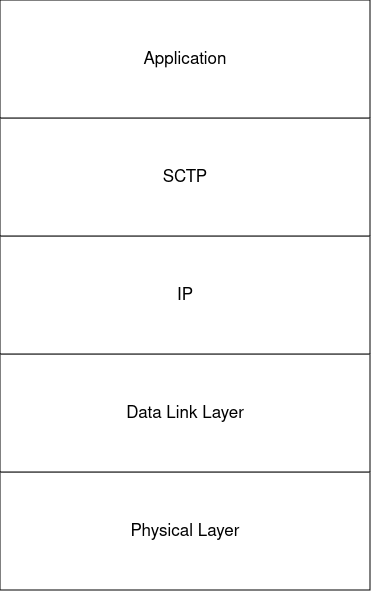
\includegraphics[width=0.35\linewidth]{figures/VisionModule_ProtocolStack.drawio(2)}
    \caption[Proposed Vision Module Protocol Stack]{Proposed Vision Module Protocol Stack}
    \label{fig:stack}
\end{figure}



\section{Proposed Vision Module}\label{sec:prop_vision}
Our proposed vision module uses computer vision techniques to extract information about obstacles within the camera's field of view. This system processes video frames to detect and track obstacles, subsequently sending messages to subscribed services with relevant information.

The module sends five types of messages: blockage, future blockage, past blockage, the location of the UE and frame processed.

The code to implement the module includes functions responsible for communication, detection and tracking, image processing, and utility functions.

%----------
Functionality Overview

    Frame Capture and Processing:
        The vision module captures frames using a camera.
        Each frame is processed to detect and track objects, utilizing techniques such as YOLO (You Only Look Once) for object detection and ArUco markers for identifying and tracking specific regions of interest.

    Obstacle Detection:
        The system identifies obstacles within the camera's field of view and determines their positions relative to the UE.
        It assesses whether these obstacles are blocking the UE or might block it in the future.

    Message Types:
        Blockage Messages: Sent when an obstacle is currently blocking the UE.
        Future Blockage Messages: Sent when an obstacle is predicted to block the UE based on its current trajectory.
        Past Blockage Messages: Sent when an obstacle that was previously blocking the UE is no longer doing so.
        UE Location Messages: Sent to provide the current location of the UE.
        Frame Processed: Sent to provide information that a frame of the video was processed.

    Communication:
        The module sends messages containing key information about detected obstacles to subscribers.
        Messages include details such as the obstacle's type, location, and the confidence level of the detection.

    Single UE Focus:
        The current implementation supports tracking and reporting information for a single UE.
%-----------
The file ObstacleDetectionReport.asn contains the specification of the set of messages created. The messages are composed of a header and a payload. The header of all messages is the same: 


\begin{table}[H]
    \caption{Components of the Message Header}
    \label{tab:header}
    \centering
    \begin{tabular}{|c|c|}
        \hline
        \textbf{Field}                     & \textbf{Description}                                                                                                                                 \\ \hline
        messageType                        & Detection algorithms must process and identify relevant obstacles within a maximum of 100ms to ensure real-time perception and decision-making.      \\ \hline
        timestamp                          & The system must send detected obstacle information to relevant network entities within 50ms to maintain near real-time data flow and responsiveness. \\ \hline
        sourceId                           & The vision module should run on hardware capable of processing video at a minimum of 30 frames per second. Suggested hardware includes:              \\ \hline
        destinationId                      & Identifies the intended recipient of the message. In this case, the xApp.                                                                                                                                                     \\ \hline
        e2InstanceId &                      Provides a unique identifier for the E2 interface instance associated with the message.                                                                                                          \\ \hline
    \end{tabular}
\end{table}

As for the content of the payload, it varies according to the type of message.
Each message requires different processing in order to extract the information required.
The following subsections present the implemented algorithm for each one of them. 

\subsection{Prediction of Blockage Messages}



\subsection{Blocking messages}

\subsection{Past Blockage}

\subsection{Location of UEs}
This message contains the location of the UEs. In order to extract such information it is required to detect the bounding boxes of the markers given for the UEs. 

The code monitors the movement of the UEs (User Equipment) and sends reports when changes are detected. This includes comparing current and previous visible ArUco IDs, buffering for changes, and sending location reports.

    Aruco IDs Comparison:
        Compare current and last visible ArUco IDs to detect changes.
    Buffering Changes:
        Use a time buffer to avoid rapid, repetitive changes.
    Sending Reports:
        Send location reports when the buffer is filled.


\section{System Design}\label{sec:design}
% review to improve
% where does the server goes? because the camera is on the gnb
This section will present the system designed to implement and evaluate the proposed solution.
The system is depicted in Figure~\ref{fig:design_arch}.
It is composed of three main logical units.
One implementing the vision module server and the 5G Core Network, the Near-RT RIC and the xApp. % may need changes
The second unit implements the mobile RAN, consisting of the gNB and the Control Application. % control application: vision module client and control of robot
The last unit implements the UE software.


\begin{figure}
    \centering
    
\includegraphics{figures/uporto-feup}
    \caption[System architecture designed for implementing and evaluating the proposed solution]{System architecture designed for implementing and evaluating the proposed solution}
    \label{fig:design_arch}
\end{figure}

The following subsections detail the hardware used in the implementation and the choices for software packages.


\subsection{Software}
This section presents the software packages used to develop the vision module and implement the 5G network.

For the Vision Module:

    System Architecture:
        A modular approach where different components (object detection, tracking, messaging) interact.
        Use of a specific object detection algorithm (e.g., YOLO) and tracking method (e.g., Deep SORT).
        Integration with the xApp via a defined communication protocol (SCTP).

    Data Flow and Interaction:
        Video frames are captured and processed in real-time.
        Detected objects and their coordinates are identified and tracked over time.
        Detected obstacles are analyzed to predict potential blockages.
        Formatted messages containing detection results are sent to the xApp.

    Component Design:
        Detection Component: Utilize YOLO for object detection.
        Tracking Component: Use Deep SORT for tracking detected objects.
        Messaging Component: Encode messages using ASN.1 and send via SCTP.


\subsubsection{OpenCV}
% revision
There are several open-source software packages available for Computer Vision in Python.
Open Source Computer Vision Library (OpenCV) is one of them.
It contains several optimized algorithms, which can be used for a variety of tasks including object detection, image processing, and real-time video analysis.
This extensive algorithmic support makes it suitable for both basic tasks and complex applications requiring advanced functionalities.
Moreover, OpenCV's well-documented API facilitates ease of use and integration into various projects, ensuring efficient development and deployment.
Unlike some other libraries that may focus on specific aspects of image processing or lack comprehensive support across different domains, OpenCV provides a solution with cross-platform compatibility, making it applicable across diverse operating systems and hardware setups.
Furthermore, OpenCV benefits from a large and active community, offering extensive resources, tutorials, and community support, which are invaluable for developers and researchers seeking assistance or collaboration in tackling complex computer vision challenges effectively and efficiently.
Therefore, OpenCV is the leading choice for robust and scalable computer vision applications.



Additionally, OpenCV is the only library who directly supports Aruco Markers.
ArUco is a widely-used open-source library for Augmented Reality (AR) applications that involves detecting and tracking augmented markers.
These markers are specially designed square or rectangular patterns with a unique binary encoding, which can be printed and placed in the physical environment.
ArUco markers are typically used in computer vision tasks to provide reference points in a scene, enabling accurate localization and tracking of objects or cameras.

OpenCV emerges as the premier choice among general computer vision libraries, distinguished by its extensive feature set, optimized performance, and robust community support.
Unlike scikit-image, which excels in image processing tasks with functions for filtering, morphology, and segmentation, OpenCV offers a broader range of over 2500 optimized algorithms spanning image and video processing, object detection, and camera calibration.
In contrast to Pillow (PIL Fork), which specializes in image format handling and basic manipulation, OpenCV provides comprehensive tools for both foundational and advanced computer vision applications.
Moreover, while SimpleCV simplifies OpenCV usage with a user-friendly interface, OpenCV's C++ backend and GPU acceleration capabilities deliver superior performance crucial for real-time processing and large-scale data operations.
OpenCV's extensive documentation, tutorials, and active community support further solidify its position as the preferred choice for developers and researchers seeking versatility, efficiency, and collaborative resources in the realm of computer vision.

In our proposed solution, OpenCV is utilized to:
\begin{itemize}
    \item \textbf{Obtain Frames:} OpenCV is used to capture video frames from the camera. It provides easy-to-use interfaces to capture and manipulate video streams from various input sources.
    \item \textbf{Detect ArUco Markers:} OpenCV includes modules for detecting ArUco markers, which are widely used in computer vision applications for camera calibration, pose estimation, and augmented reality. In our solution, these markers help in identifying the UEs without the need to train the YOLO model to perceive such objects. 
\end{itemize}

\subsubsection{Ultralytics YOLO}
Ultralytics YOLO (You Only Look Once) is a state-of-the-art, real-time object detection system.
It is known for its speed and accuracy, making it suitable for applications that require fast and reliable object detection and tracking.

In our proposed solution, Ultralytics YOLO is employed to:
\begin{itemize}
    \item \textbf{Detection:} YOLO is used to detect various objects in the frames captured by the camera. Its real-time capabilities allow for the immediate identification of obstacles within the field of view.
    \item \textbf{Tracking:} YOLO’s tracking module is used to keep track of detected objects over successive frames. This is crucial for maintaining the continuity of object identification and for predicting future positions of the obstacles. %BOTSORT and BYTETRACK
\end{itemize}

The combination of OpenCV and Ultralytics YOLO allows for robust detection, tracking, and communication functionalities in our vision module. OpenCV handles the initial capture and processing of video frames, while YOLO performs the real-time detection and tracking of objects. This integrated approach ensures that the vision module can effectively monitor and report on obstacles, providing key information to subscribed services.

\subsubsection{ASN1Tools and ASN1C}

\subsubsection{5G Core Network, 5G gNB, and 5G UE}
The main open-source 5G software packages for implementing an O-RAN based architecture are OAI \cite[]{} and srsRAN \cite[]{}. For our system, we chose OAI because it provides all the necessary components to deploy a 5G standalone network, including both the RAN and Core networks. In contrast, srsRAN only supports the deployment of the RAN, requiring an additional software package, such as OAI, to implement the Core network.

\subsubsection{Near-RT RIC}
The main open-source software packages able to implement a Near-RT RIC are Mosaic5G’s FlexRIC \cite[]{} and  O-RAN Software Community’s Near-RT RIC \cite[]{}.
The first was chosen more suitable for our application due to the fact that lightweight application, launched from an executable file.

\subsection{Hardware}
\subsubsection{Core Network, FlexRIC, Computer Vision module and gNB}
The OAI Core Network, FlexRIC,the Computer Vision module and the gNB were deployed in a laptop Acer Aspire A715-74G\@.
The OAI Core was deployed using Docker containers, requiring 4 cores CPU, 16GB of RAM and a minimum of 1.5GB free storage for the docker images.
As for FlexRIC, it does not have hardware requirements listed, but while deploying it was noticed that it is not resource intensive, sufficing the same ones required for the Core Network.
The xApp was deployed alongside FlexRIC in order to assure reduced latency between the two components.
Also,  the way interface E42 is implemented requires them to be running in the same computing unit.
As for the gNB, the hardware recommended are 8 physical CPU cores and 32 GB of RAM\@.
While the laptop used did not fulfill these requirements, it has proven sufficient to run the OAI gNB software, as it was noted before in \ref{}. % ref to dissertation of gonçalo

As for the Computer Vision Module, the minimal hardware requirement is a CUDA-compatible GPU ~\cite{}, for Ultralytics YOLO model to properly run.
Given that for our solution pre-trained model has proven enough to accurately detect and track objects, we did not worried about fulfilling the
%%%%%%%%%%%% finalize



Table ~\ref{tab:specs_pc} presents the specification of the computer.

\begin{table}[H]
    \begin{tabular}{|c|c|}
        \hline
        \textbf{Specification} & \textbf{Details} \\ \hline
        Processor                      &           Intel(R) Core(TM) i5-9300H CPU @ 2.40GHz   \\ \hline
        RAM                      &          16GB        \\ \hline
        Disk                      &   2 SSDs  512GB and 256GB         \\ \hline
        GPU                     &   GeForce GTX 1050 (3GB)      \\ \hline
        Operational System & Ubuntu 22.04.4 LTS                  \\ \hline
    \end{tabular}\label{tab:specs_pc}
\end{table}

For the Computer Vision Module, we opted to use a webcam due to its simplicity and ease of integration.
The chosen webcam, a model LL-4196, offers Full HD (1920 x 1080 Pixels) resolution and supports a frame rate of 30 FPS\@.
This ensures that the video feed acquired is of high quality, providing sufficient detail and smooth motion necessary for accurate computer vision processing.
The camera connects to the computer using a USB 2.0 interface.
The specifications of the camera are sufficient for the system to detect and track movements and objects within the environment, assuring the efficient operation of the Computer Vision Module.
% why? velocity constant , processing of frame


Deploying the gNB and the UE in two different host computers implicates the use of Software-Defined Radio (SDR) in order to establish a 5G connection between the gNB and the UE.
OAI recommends the use of three SDR models: USRP B210, USRP N300 and USRP X300\@ \cite{}. %https://gitlab.eurecom.fr/oai/openairinterface5g/-/blob/develop/doc/NR_SA_Tutorial_OAI_nrUE.md
For our implementation, we have selected the first since it is cost-effective and a popularity across the community.
This model uses a USB 3.0 interface to connect to the computer acting as a processing unit.
The SDR was equipped with two W5208K dipole antennas.
Figure \ref{} shows the two SDRs with their respective antennas.
We have selected 3.6GHz as the carrier frequency for the 5G RAN.

\subsubsection{UE}
The UE was deployed in HP EliteBook 840 Laptop.
The hardware requirements for the deployment of the UE are 8 cores and 8GB of RAM\@.
Table~\ref{tab:specs_pc_ue} depicts the specification of the computer responsible for the UE\@.

\begin{table}[H]
    \begin{tabular}{|c|c|}
        \hline
        \textbf{Specification} & \textbf{Details} \\ \hline
        Processor                      &              \\ \hline
        RAM                      &          8GB        \\ \hline
        Disk                      &   2 SSDs  512GB and 256GB         \\ \hline
        GPU                     &   None                \\ \hline
        Operational System & Ubuntu 22.04.4 LTS                  \\ \hline  %  check
    \end{tabular}\label{tab:specs_pc_ue}
\end{table}


\section{System Implementation}\label{sec:impl}

For the Vision Module:

    Coding:
        Implementing object detection and tracking using YOLO and BoT-SORT algorithms.
        Implementing ArUCO marker detection using OpenCV
        Developing the communication interface using SCTP and ASN.1 for message encoding.
        Handle video input, process each frame, and generate output messages.

    Testing:
        Running unit tests to ensure each component (detection, tracking, messaging) works as intended.
        Conducting integration tests to verify that components interact correctly.
        Performing system tests with both pre-recorded videos and real-time captures to ensure the module meets the specified performance criteria (e.g., processing speed, accuracy).

    Deployment:
        Deploying the vision module on the specified hardware.
        Monitoring performance in real-time scenarios to ensure it meets the defined requirements.
        Making adjustments and optimizations based on observed performance and feedback.

\subsection{OAI 5G Core Network}
OAI offers three methods for implementing the Core Network: bare-metal installation or virtual machines, automated deployment of network functions (NFs) in Docker containers using Docker-Compose, and cloud-native deployment using Helm Chart on OpenShift or Kubernetes clusters ~\cite{}.
Choosing Docker for deployment simplifies the process by encapsulating network functions in containers, making them easier to manage, scale, and automate, which enhances the overall efficiency and flexibility of the network infrastructure.

Besides that, the Core can be implemented in two scenarios.
We chose scenario I , since it contains the minimum components necessary in order to test end to end connectivity between the nodes.
This scenario contains 8 containers.
python3 core-network.py --type start-basic --scenario 1
- Scenario I:  AMF, SMF, UPF (SPGWU), NRF, UDM, UDR, AUSF, MYSQL


\subsection{OAI gNB}
\subsection{OAI 5G UE}
\subsection{FlexRIC}

% what else?

\section{Summary}






